\documentclass{article}

\usepackage{a4wide}
\usepackage[utf8]{inputenc}
\usepackage[T1]{fontenc}
\usepackage[french]{babel}
\usepackage[babel=true]{csquotes} % guillemets français
\usepackage{graphicx}
\graphicspath{{Images/}}
\usepackage{color}
\usepackage{hyperref}
\hypersetup{colorlinks,linkcolor=,urlcolor=blue}

\usepackage{amsmath}
\usepackage{amssymb}


\title{Prise de notes}
\author{Said Ismael, M1 Informatique}
\date{\today}

\begin{document}

\maketitle % pour écrire le titre

% PAGE BLANCHE

\newpage
\thispagestyle{empty}
\mbox{}
\newpage

% FIN PAGE BLANCHE



% TABLE DES MATIERES
\tableofcontents
\newpage

% PAGE BLANCHE


\begin{abstract}
  Travail réalisé avec le \textit{Cirad}~\cite{coursera}.


  Lien vers mon \textit{github}~\cite{github}
\end{abstract}


\section{Introduction}
Le travail demandé consiste à concevoir une base de données relationnelle.
\section{Modèle entité-association}
\subsection{Schéma entité-association}
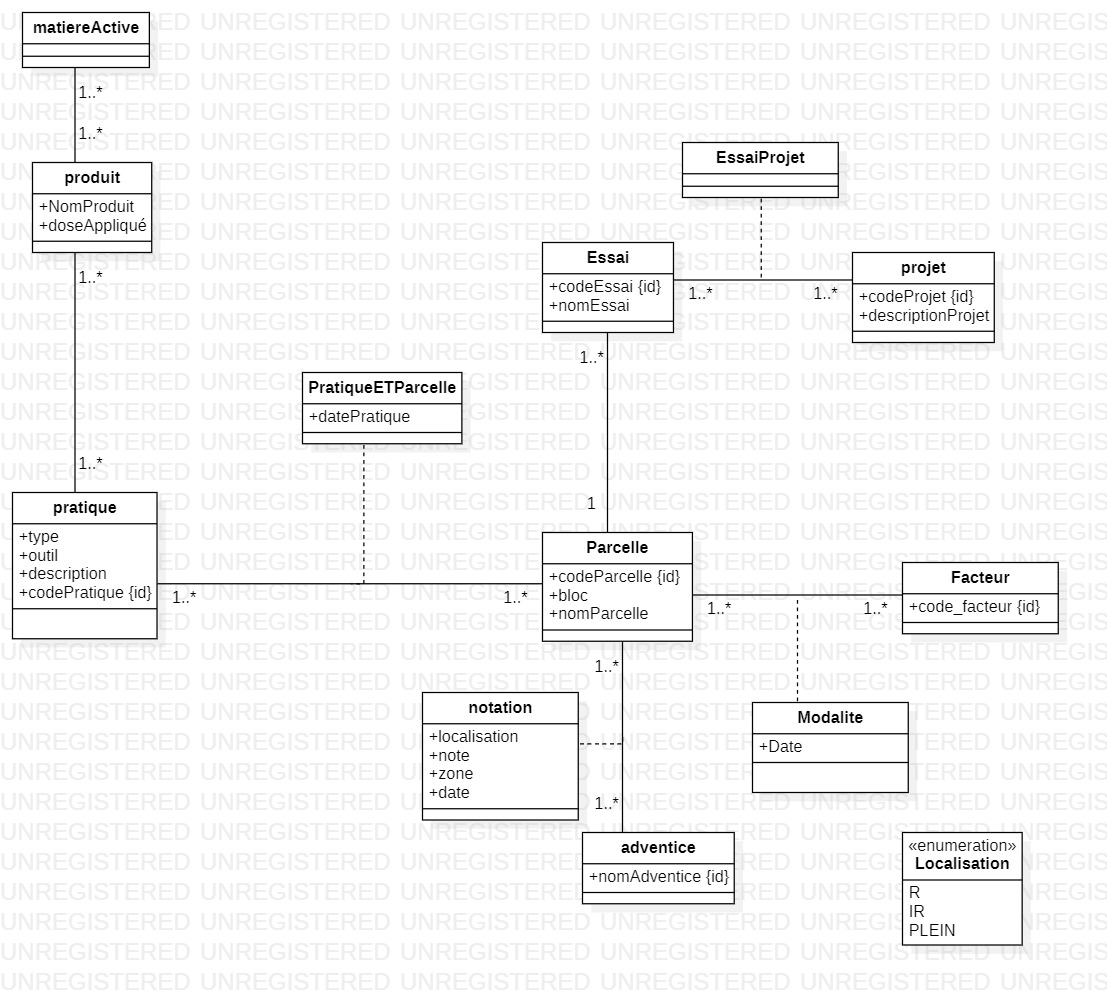
\includegraphics[scale=0.35]{Main.jpg}


\subsection{Définition des termes}

\textbf{Essai:} \textit{à définir} 

\textbf{Modalité:} \textit{à définir}

\textbf{Parcelle:} \textit{à définir}

\textbf{Adventice:} \textit{à définir}

\textbf{Facteur:} \textit{à définir}

\textbf{Pratique:} \textit{à définir}


\subsection{Sémantique des relations}
\begin{itemize}
  \item Un essai appartient au minimum à un seul projet et au maximum à n projets 
  \item Un Projet contient au minimum un seul essai et au maximum n essais
  \item Un essai met en jeu au minimum une seule parcelle et au maximum n parcelles
  \item Une parcelle est le sujet de un seul et unique essai
  \item Une adventice peut se retrouver au minimum sur aucune et au maximum sur n parcelles
  \item Une parcelle peut contenir au minimum aucune adventice et au maximim n adventices
  \item Un un ou plusieurs facteurs peuvent être appliquées à une parcelle.
  \item Une parcelle est caractérisée par un ou plusieurs facteurs
\end{itemize}


\section{modèle relationnel}
\subsection{Tables}
\begin{itemize}
  \item projet(\underline{codeprojet},descriptionprojet)  
  \item essaie(\underline{codeessai},nomessai)
  \item essaiprojet(\#codeessai,\#codeprojet,date)
  \item adventice(\underline{nomAdventice}) 
   % La clé primaire de Essai va migrer vers Parcelle
  \item parcelle(\underline{codeparcelle},bloc,nomparcelle,\#codeessai)
  \item notation(\#codeparcelle,\#nomadventice,localisation,note,zone,date)
  \item facteur(\underline{codefacteur},descriptionfacteur)
  \item modalite(\#codeparcelle,\#codefacteur,date)
  \item pratiqueagricole(\underline{codepratique},type,outil,description)
  \item realisation(\#codeparcelle,\#datepratique,date)
  \item produit(\underline{nomproduit},doseapplique)
  \item matiereactive(\underline{codematiereactive},dosagemaximal)
\end{itemize}
% Ne pas utiliser les tables: Pratique, produit,matiere active et pratiqueParcelle pour l'instant




%%% La bibliographie:
\bibliographystyle{plain}
\bibliography{ma_biblio}


\end{document}
